\documentclass[a4paper, 12pt]{article}
\usepackage[top=2cm, bottom=2cm, left=1.5cm, right=1.5cm]{geometry}
\usepackage{graphicx}
\usepackage{float}
\usepackage{pgfplots}


\begin{document}
	\begin{center}
		Universidade Federal do Rio Grande do Norte
		
		Departamento de Engenharia da Computação e Automação
		
		DCA3703 - Programação Paralela
		
		\textbf{Tarefa 4 - Aplicações limitadas por memória ou CPU}
		
		\textbf{Aluno:} Daniel Bruno Trindade da Silva
	\end{center}
	
	\section{Introdução}
	
	\hspace{.7cm}A computação paralela tem se tornado uma estratégia essencial para melhorar o desempenho de programas, especialmente com a popularização de processadores com múltiplos núcleos. O OpenMP (Open Multi-Processing) é uma API amplamente utilizada para programação paralela em sistemas com memória compartilhada, permitindo a distribuição de tarefas entre múltiplas threads de forma simples e eficiente. Este relatório apresenta a implementação e análise de dois programas paralelos desenvolvidos em linguagem C com OpenMP: um limitado por memória (memory-bound), baseado em somas simples entre vetores, e outro limitado por processamento (compute-bound), com operações matemáticas intensivas.
	
	O objetivo principal é avaliar o impacto da paralelização com a diretiva \texttt{\#pragma omp parallel for} no tempo de execução dos programas, variando o número de threads utilizadas. A partir dos experimentos, são observadas as situações em que o desempenho melhora, se estabiliza ou até mesmo piora, permitindo uma reflexão sobre os efeitos do multithreading de hardware em diferentes cenários. Essa análise contribui para a compreensão dos limites e vantagens da programação paralela, considerando o perfil computacional das aplicações.
	
	\section{Metodologia}
	
	\hspace{.7cm}Realizamos a implementação de dois programas em C, o primeiro deles tem como objetivo realizar somas simples para simular uma carga de trabalho limitada pelo acesso a memória (memory-bound). Ele aloca dinamicamente um vetor de 100 milhões de elementos do tipo double e realiza uma operação simples de escrita: atribuir a cada posição do vetor o valor i + 2, onde i é o índice da iteração. A paralelização é feita com a diretiva \texttt{\#pragma omp parallel} for, permitindo que múltiplas threads realizem essas atribuições em paralelo.
	
	O tempo de execução é medido com a função \texttt{omp\_get\_wtime()}, antes e depois do laço paralelo. Como a operação executada em cada iteração é computacionalmente simples, o desempenho do programa depende principalmente da taxa de leitura e escrita na memória principal. Esse tipo de programa evidencia os limites do ganho de desempenho com o aumento do número de threads, já que o gargalo está na largura de banda da memória, e não na capacidade de cálculo da CPU.
	
	Assim ficou nosso código:
	
	\begin{verbatim}
		#include <stdio.h>
		#include <stdlib.h>
		#include <omp.h>
		
		#define SIZE 100000000
		
		int main() {
			
			double *a = (double *)malloc(SIZE * sizeof(double));
			double start, end;
			
			start = omp_get_wtime();
			#pragma omp parallel for
			for (int i = 0; i < SIZE; i++) {
				a[i] = i+2;
			}
			end = omp_get_wtime();
			
			printf("Tempo de execução (Memory-bound): %f segundos\n", end - start);
			
			free(a);
			
			return 0;
		}
	\end{verbatim}
	
	O segundo programa desenvolvido simula uma carga de trabalho limitada pela capacidade de processamento da CPU (CPU-bound). Ele realiza 100 milhões de operações matemáticas intensivas, envolvendo funções como sin, cos e sqrt, seguidas de uma divisão. Essas operações são realizadas dentro de um laço for paralelo, utilizando a diretiva \texttt{\#pragma omp parallel for} com uma cláusula de reduction para somar corretamente os resultados parciais de cada thread na variável \texttt{result}.
	
	O tempo de execução também é medido com \texttt{omp\_get\_wtime()}. Diferente do programa memory-bound, aqui o gargalo está no tempo necessário para realizar os cálculos matemáticos complexos, que demandam mais ciclos de CPU. Esse tipo de programa permite observar como o desempenho pode escalar com múltiplas threads até certo ponto, mas também evidencia como o aumento de concorrência pode gerar competição por recursos internos da CPU, como unidades de ponto flutuante e cache, o que pode limitar os ganhos ou até causar perda de desempenho.
	
	O código para essa programa ficou assim:
	
	\begin{verbatim}
		#include <stdio.h>
		#include <math.h>
		#include <omp.h>
		
		#define SIZE 100000000
		
		int main() {
			double result = 0.0;
			int i;
			double start, end;
			
			start = omp_get_wtime();
			#pragma omp parallel for reduction(+:result)
			for (i = 0; i < SIZE; i++) {
				result += sin(i) * cos(sqrt(i)) / (i + 1.0);
			}
			end = omp_get_wtime();
			
			printf("Tempo de execução (CPU-bound): %f segundos\n", end - start);
			printf("Resultado final: %f\n", result);
			
			return 0;
		}
	\end{verbatim}
	
		Para execução de ambos os programas (memory bound e cpu bound) utilizamos a diretiva \texttt{OMP\_NUM\_THREADS=\textit{n}} onde \textit{n} é o número de threads que sera utilizado para execução. Nesse estudo aumentaremos o valor de \textit{n} progressivamente afim de verificar até que ponto temos ganho de desempenho.
		
		Como os resultados desse experimento dependem diretamente do hardware utilizado se faz importante mencionar que os códigos estão sendo executado em um computador com a seguinte configuração:
		
		\begin{itemize}
			\item \textbf{Processador:} Intel I3 10100F 
				\begin{itemize}
					\item Núcleos: 4
					\item Threads: 8
				\end{itemize}
			\item \textbf{Memoria RAM:} 16 gigas
				\begin{itemize}
					\item Frequência: 2400Hz
				\end{itemize}	
		\end{itemize}
		
	\section{Resultados}
	
	Primeiro vamos conferir os resultados obtidos no código do Memory Bound. Executamos o código por 10 vezes sempre aumentando o número de threads, ou seja, começamos com 1 thread e fomo até 10.
	
	Obtivemos o seguinte resultado:
		
	\begin{table}[h]
		\centering
		\begin{tabular}{|c|c|c|c|c|c|c|c|c|c|c|}
			\hline
			\textbf{Threads} & 1 & 2 & 3 & 4 & 5 & 6 & 7 & 8 & 9 & 10 \\
			\hline
			\textbf{Tempo (s)} & 0.3745 & 0.2012 & 0.1366 & 0.1085 & 0.0999 & 0.0874 & 0.0757 & 0.0868 & 0.0817 & 0.0794 \\
			\hline
		\end{tabular}
		\caption{Tempo de execução do programa \textbf{memory-bound} para diferentes números de threads}
		\label{tab:memory-bound}
	\end{table}
	
	\begin{figure}[h]
		\centering
		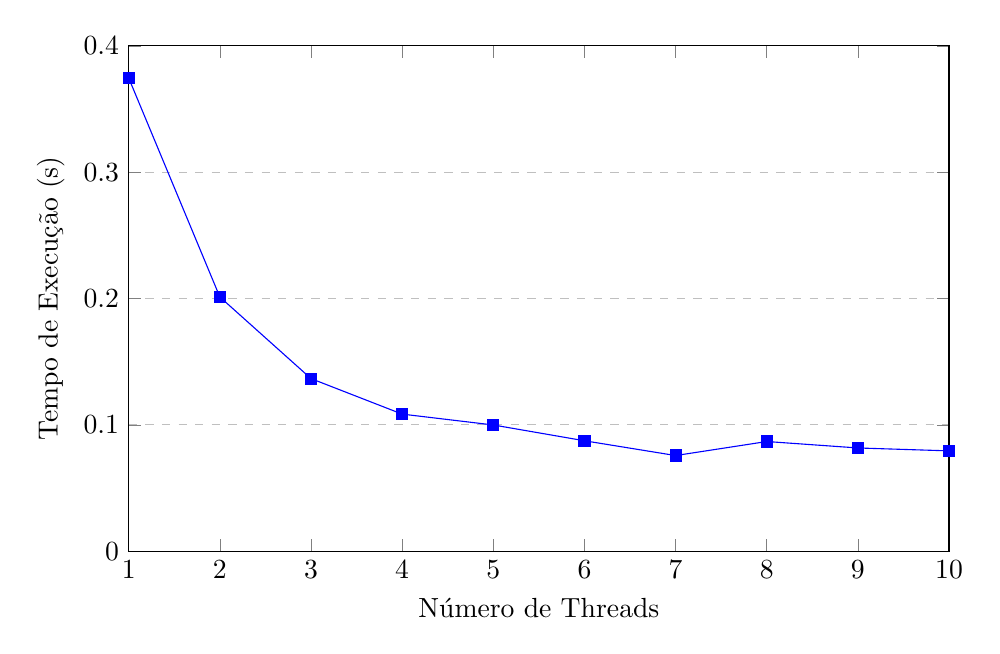
\begin{tikzpicture}
			\begin{axis}[
				xlabel={Número de Threads},
				ylabel={Tempo de Execução (s)},
				xmin=1, xmax=10,
				ymin=0, ymax=0.4,
				xtick={1,2,3,4,5,6,7,8,9,10},
				ymajorgrids=true,
				grid style=dashed,
				width=12cm, height=8cm
				]
				\addplot[color=blue, mark=square*] coordinates {
					(1,0.3745) (2,0.2012) (3,0.1366) (4,0.1085) (5,0.0999)
					(6,0.0874) (7,0.0757) (8,0.0868) (9,0.0817) (10,0.0794)
				};
			\end{axis}
		\end{tikzpicture}
		\caption{Desempenho do programa *memory-bound* variando o número de threads}
		\label{fig:memory-bound}
	\end{figure}
	
	
	
\end{document}